\documentclass{beamer}

% For more themes, color themes and font themes, see:
% http://deic.uab.es/~iblanes/beamer_gallery/index_by_theme.html
%
\mode<presentation>
{
  \usetheme{Madrid}       % or try default, Darmstadt, Warsaw, ...
  \usecolortheme{default} % or try albatross, beaver, crane, ...
  \usefonttheme{serif}    % or try default, structurebold, ...
  \setbeamertemplate{navigation symbols}{}
  \setbeamertemplate{caption}[numbered]
} 

\usepackage{tikz}
\usetikzlibrary{decorations.markings,angles}
\usepackage{tikz-3dplot} 

\usepackage{amsmath}


\begin{document}

\newcommand{\tikzAngleOfLine}{\tikz@AngleOfLine}
  \def\tikz@AngleOfLine(#1)(#2)#3{%
  \pgfmathanglebetweenpoints{%
    \pgfpointanchor{#1}{center}}{%
    \pgfpointanchor{#2}{center}}
  \pgfmathsetmacro{#3}{\pgfmathresult}%
  }



\begin{frame}{Poynting flux}

\bf{MHD eqs} 
 
\begin{figure}[H]
 \centering
 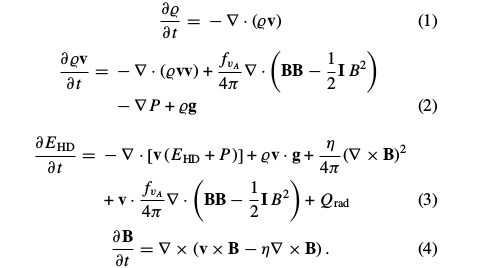
\includegraphics[scale=0.6]{eqs.png}
\end{figure}



\end{frame}

\begin{frame}{Poynting flux}

\begin{equation} \nonumber
\vec{P} =  \vec{E} \times \vec{B}   =  (- \vec{v} \times \vec{B}  + \eta \nabla \times \vec{B}) \times \vec{B}
\end{equation}

\begin{equation} \nonumber
E_{mag} = \frac{B^2}{8 \pi} , \;\;\;\; \;\;\;\; \;\;\;\;  \vec{j} = \frac{1}{4 \pi} \nabla \times \vec{B}
\end{equation}

\begin{equation} \nonumber
\frac{\partial E_{mag}}{\partial t} + \frac{1}{4 \pi} \nabla \cdot \vec{P} = -\vec{j} \cdot \vec{E}
\end{equation}

%\begin{equation} \nonumber
%\vec{P} =  4 \pi \vec{v} E_{mag} -  \vec{B}(\vec{v} \cdot \vec{B}) + 
%  \eta (  \nabla \times \vec{B})  \times \vec{B} 
%\end{equation}


\begin{equation} \nonumber
\vec{j} \cdot \vec{E} = \vec{v} \cdot \left( \vec{j} \times \vec{B} \right) + \frac{\eta}{4 \pi} \left ( \nabla \times \vec{B} \right )^2
\end{equation}

\end{frame}

\begin{frame}{Boundary conditions used here}

{\bf horizontal}: periodic

{\bf vertical}: 

\begin{itemize}

\item hydrodynamical variables:

All three mass flux components are symmetric with
respect to the boundary. We decompose the gas pressure
into mean pressure and fluctuation.  The
mean pressure is extrapolated into the ghost cells such
that its value at the boundary is fixed, while the pressure
fluctuations are damped in the ghost cells.

\item magnetic field:

\begin{itemize}
\item bottom
\begin{itemize}

\item O16bM: symmetric
\item Z16M: zero
 

\end{itemize}
\item top:  potential field extrapolation
\end{itemize}
\end{itemize}

\end{frame}

\begin{frame}{Comparison of the Poynting flux for the simulations O16bM (solid) and Z16M (dashed)}

\begin{figure}[H]
 \centering
 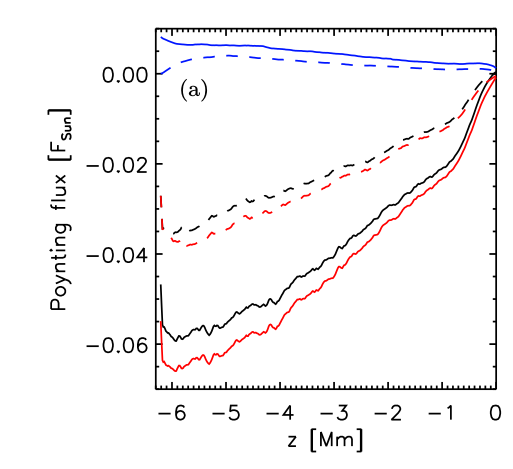
\includegraphics[scale=0.3]{poynting1.png}
	\caption{Black lines show the horizontally
averaged Poynting flux, blue and red lines present the contributions from up- and downflows}
\end{figure}

\end{frame}

\begin{frame}

\begin{itemize}
\item z component averaged in horizontal plane (horizontal component = 0 because of symmetry?), 
normalized by solar photospheric energy flux
\item bottom domain, solid line: upflow - BC open makes flux enter the domain, but downflow flux = 6 * upflow flux
\item dashed line: bottom upflow = 0(BC def) , but z $>$ -5,-4 Mm upward directed UPFLOW Poynting flux, 
almost identical contribution (as solid line) for BOTH upward and downward flow ??
\end{itemize}

\end{frame}
\begin{frame}{Comparison of energy loss rate: $-\frac{P(z)}{\int_z^{z_{top}}{E_{mag} dz }}$   for the simulations O16bM (solid) and Z16M (dashed)}

\begin{figure}[H]
 \centering
 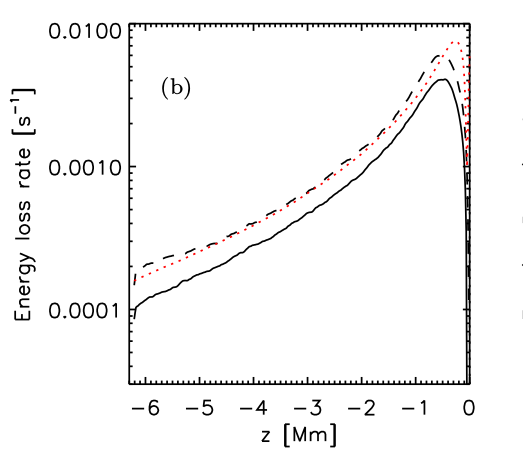
\includegraphics[scale=0.3]{poynting2.png}
	\caption{Energy loss rate due to the Poynting flux. The
red dotted line indicates a convective overturning rate: $\frac{{v_z}_{rms}}{H_{\rho}}$}
\end{figure}

\end{frame}

\begin{frame}

\begin{itemize}
\item integration in the domain above a height z
\item flux close to 0 at the top boundary
\item dashed line: magnetic loss  rate 1.8 times higher (log scale) , profile  agrees with the red line (smaller Pz, but much smaller magnetic energy: about 4 times)
\item magnetic energy loss due to overturnig convection (red line) has a slow timescale: $\frac{H_{\rho}}{{v_z}_{rms}}$
\item dynamo growth rate $\gamma >> \frac{{v_z}_{rms}}{H_{\rho}}$ (kinematic growth phase) achieved always with high resolution($\Delta x \le 8km$), low resolution(16 km here) only in in the bottom part,
not in the photosphere
\item non linear saturation phase:  $\gamma \approx \frac{{v_z}_{rms}}{H_{\rho}}$ bottom BCs matter
\item dashed line: maximum energy loss at the bottom boundary $\implies$ the lower limit(small saturation field strength)  for an efficient dynamo (solid line below dashed: more efficient) 
\end{itemize}

\end{frame}

\begin{frame}{Comparison of the energy lost by the Poynting flux to the
energy converted via the Lorentz force:  $\frac{P(z)}{\int_z^{z_{top}}{ \vec{v} \cdot \left( \vec{j} \times \vec{B} \right)dz }}$ for the simulations O16bM (solid) and Z16M (dashed)}

\begin{figure}[H]
 \centering
 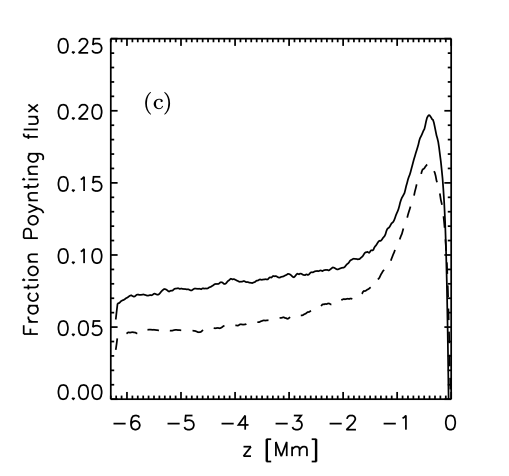
\includegraphics[scale=0.3]{poynting3.png}
	\caption{Fraction of energy transported by the Poynting flux relative to energy converted by the Lorentz
force}
\end{figure}

\end{frame}


\begin{frame}
\begin{itemize}
\item dashed line below solid line because saturation affects more $\vec{v} \cdot \left( \vec{j} \times \vec{B} \right)$ than $-(\vec{v} \times \vec{B}) \times \vec{B}$ (part of $\vec{P}$ ) ($\implies$ this fraction bigger because of saturation)
and stronger saturation effect in solid line
\item  $\int_{z_{bottom}}^{z_{top}}{E_{mag} dz}$ 4 times bigger in solid line than dashed, 
\item but $\int_{z_{bottom}}^{z_{top}}{ \vec{v} \cdot \left( \vec{j} \times \vec{B} \right)dz }$ comparable, 50\% of the energy
converted by pressure/buoyancy forces in the domain, 80\% of the
energy flux through the domain
\item Most of
the energy converted from kinetic to magnetic is preferentially
dissipated in downflow regions, while work against the Lorentz
force reduces the kinetic energy there. This changes the overall
balance of the convective energy transport by reducing the
contribution from the kinetic energy flux. We find in a non-
magnetic convection simulation in 6 Mm depth a downward
directed kinetic energy flux of about -0.3 Fs , this value is
reduced to −0.2 Fs in simulation O16bM
\end{itemize}
\end{frame}


\begin{frame}{Dependence on domain size and resolution}
\begin{itemize}
\item small scale {\bf grid resolution dependence}

Recently, Hotta et al. (2014) presented small-scale dynamo
simulations in a global setup covering the convection zone
up to 7 Mm beneath the photosphere. Using a similar numerical
 approach, but a substantially lower grid spacing of
1100 km horizontally and 375 km vertically, they were able to
maintain a field with 0.15-0.25 $B_{eq}$ throughout the convection

Overall field strength reached (their
field near the top boundary falls short of our values by a factor
of four, which is reflected in an energy conversion rate more
than a factor of 10 lower)

\item {\bf small scale - large scale difference}

Integrated over the entire convection
zone, the energy conversion rate
extracted from large-scale mean
flows in mean field dynamo models (Rempel 2006), as well
as three-dimensional global dynamo simulations (Nelson et al.
2013), is about two orders of magnitude smaller.

\end{itemize}

\end{frame}

\begin{frame}{Horizontal Magnetic Field above $\tau$ = 1 for O16bM }

\begin{figure}[H]
 \centering
 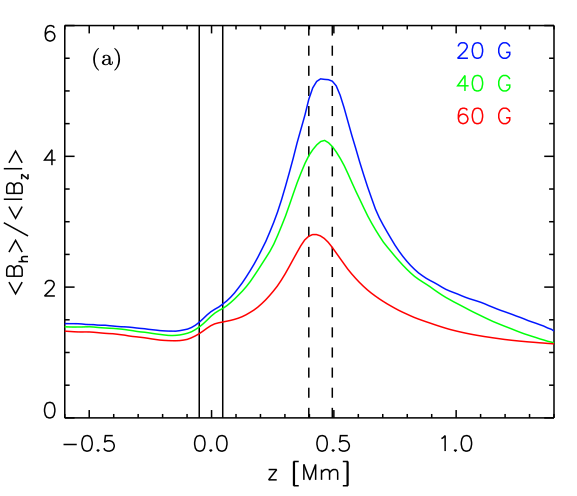
\includegraphics[scale=0.3]{img381.png}
	\caption{Ratio of horizontal to vertical field strength as a function of height. Different colors refer to simulations with the average vertical field strength at $\tau$ = 1
as indicated. The ratio of the horizontal to vertical field has a maximum at about 450 km above $\tau$ = 1 and is strongly dependent on the overall field strength of the
simulation and decreases with increasing field strength. }
\end{figure}

\end{frame}

\begin{frame}{Horizontal Magnetic Field above $\tau$ = 1 for O16bM}

\begin{figure}[H]
 \centering
 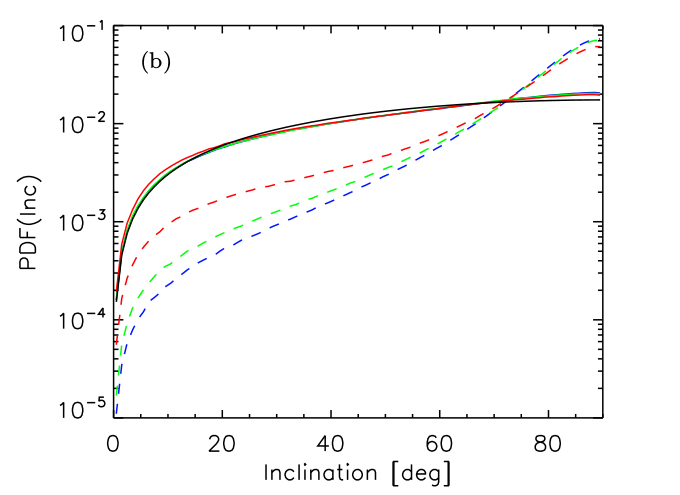
\includegraphics[scale=0.3]{img382.png}
	\caption{ Probability distribution functions for the field inclination with respect to the vertical. Solid lines refer to
the deep photosphere around $\tau$ = 1, and dashed lines to about 450 km height. 
The black solid line indicates an isotropic distribution of field inclinations(agreement with solid lines).}
\end{figure}

\end{frame}

\begin{frame}{Horizontal Magnetic Field above $\tau$ = 1 for O16bM}

\begin{figure}[H]
 \centering
 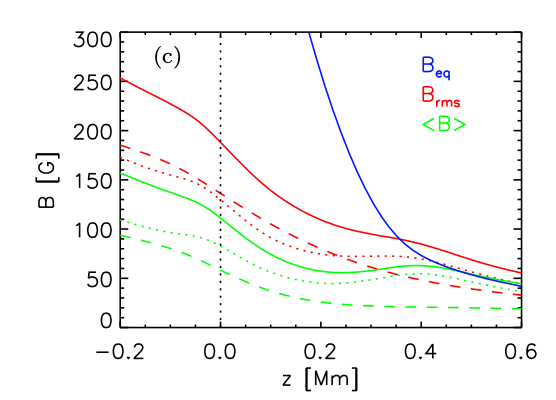
\includegraphics[scale=0.3]{img383.png}
	\caption{the magnetic field structure at the photosphere. Red (green) lines indicate
the rms (mean) field strengths, while blue lines show the equipartition field strength. The meaning of the line styles: dashed
(dotted) lines refer to the corresponding averages of vertical (horizontal) field components}
\end{figure}

\end{frame}


\begin{frame}{}
4.4 Distribution function: kG field concentrations
\end{frame}

\begin{frame}{PDF  robust $\impliedby $ no dependence on resolution}

\begin{figure}[H]
 \centering
 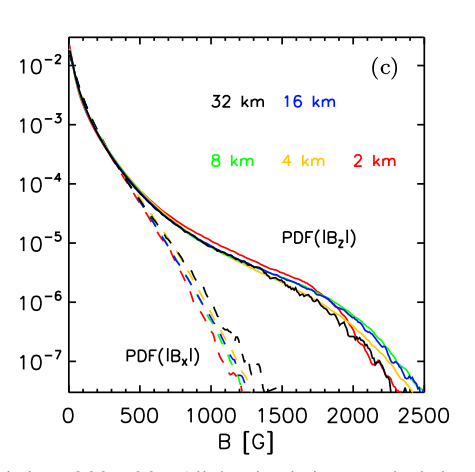
\includegraphics[scale=0.3]{img44-1.png}
	\caption{
Panel (c) shows the PDF for $\lvert$B x $\rvert$ and $\lvert$B z $\rvert$ at $\tau$ = 1. We do
not see a systematic dependence on resolution, differences for
stronger field are mostly realization noise. For fields with less
than 500 G strength the PDFs for $\lvert$B x $\rvert$ and $\lvert$B z $\rvert$ are essentially
identical. Note that we show here the PDFs for the absolute values of the field components since the simulations do not have
any net magnetic flux, leading to symmetric PDFs with respect
to B = 0.}
\end{figure}




\end{frame}


\begin{frame}{The shape of the PDF depends on field strength and domain size }
\begin{itemize}
\item for $<\lvert$Bz $\rvert>$  80 G we find that 50\% of the energy
comes from fields with less than 500 G, kG field concentrations
contribute about 16\% to the total energy 
\item weaker field 60G  energy from kG field concentrations drops to 9\%
\item 60G, larger domain it increases to 23\%
\item the filling factor of the kG field
concentrations (area with field $<\lvert$B $\rvert>$ $>$ 1kG discussed in 3.4) is strongly field strength dependent. More than $<\lvert$B z $\rvert>$ 	 $\approx$ 30 - 40 G is required at $\tau$ = 1 before they form and the
filling factor increases steeply as the field strength increases
beyond that threshold 
\end{itemize}

\end{frame}

\begin{frame}{The filling factor}
\begin{figure}[H]
 \centering
 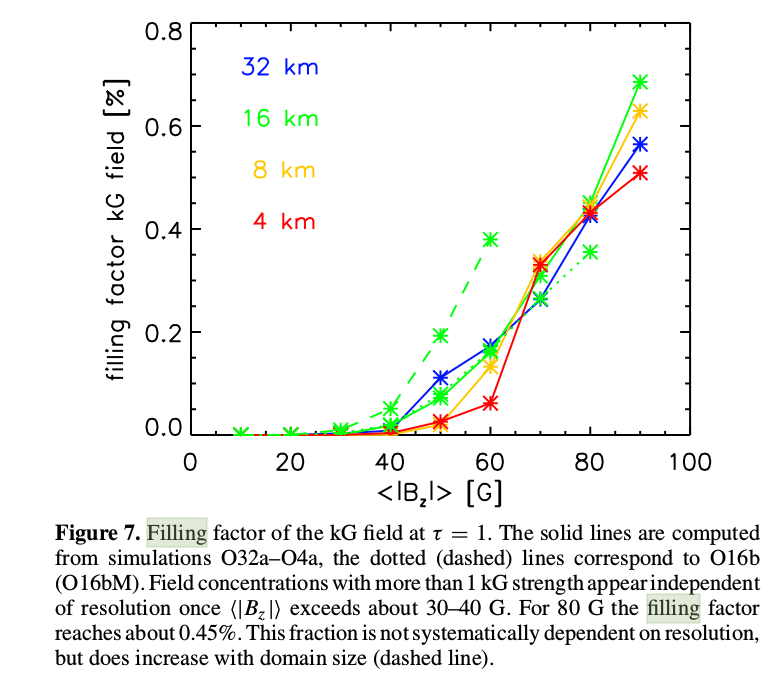
\includegraphics[scale=0.3]{img44-3.png}
\end{figure}

\end{frame}


\begin{frame}{Comparing PDF for horizontal and vertical field}

\begin{itemize}
\item Comparing the shape of normalized
PDFs for vertical and horizontal field components, we find
that the PDFs for the vertical field in the photosphere deviate
substantially from those of horizontal field, as well as vertical
field beneath the photosphere

\item This is a strong
hint for the presence of a convective intensification mechanism
(Schüssler 1990) that is restricted to the photosphere and mostly
affects the vertical field
\end{itemize}
\end{frame}


\begin{frame}{Comparing PDF for horizontal and vertical field}
\begin{figure}[H]
 \centering
 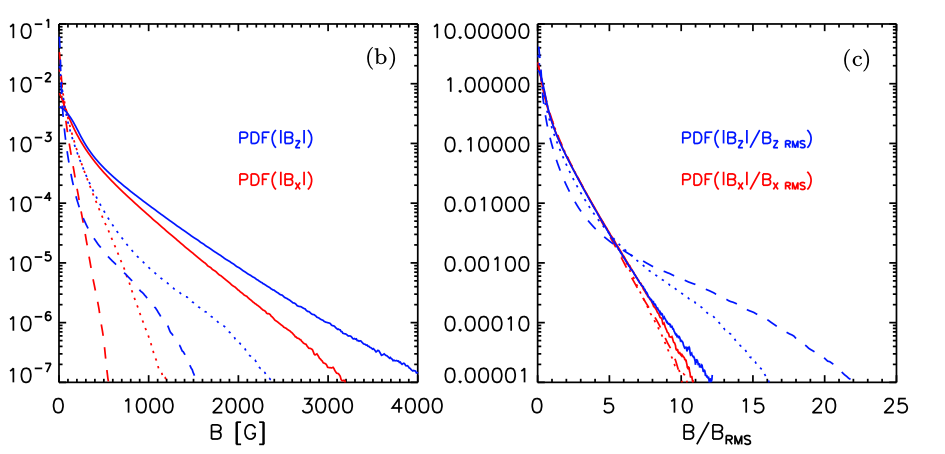
\includegraphics[scale=0.3]{img44-2.png}
	\caption{
(b), (c) probability distribution functions for $\lvert$B x $\rvert$ and $\lvert$B z $\rvert$ for three different height levels in simulation O4a. Solid
lines show quantities in 1 Mm depth, dotted lines on the $\tau$ = 1, and dashed lines on the $\tau$ = 0.01 levels. Panel (c) compares normalized PDFs, which allow for a direct
comparison of the shape regardless of field strength}
\end{figure}

\end{frame}

\begin{frame}{Strong magnetic field at $\tau$ = 1 (up to 2.5 kG)}

\begin{itemize}

\item not organized
in the form of flux tubes, organized in sheets, often with alternating polarities. The kG flux
concentrations are small knots along these sheets in which the
field strength is increased temporarily due to dynamical effects
\item it does not have a preferred
scale around 100 km.  We find the kG flux concentrations down to the smallest scales
we can resolve 
\item The kG field present in our simulations does
not produce a distinct feature in the PDFs like a secondary peak
around kG field strength, which is found in many observations.

These observation also indicate that the second
peak is possibly caused by contributions from network field and
may not be present for an inter-network field alone
 
\end{itemize}
\end{frame}

\end{document}
